
\documentclass[border=1pt]{standalone}
\usepackage[T1]{fontenc}
\usepackage{newtxtext}
\usepackage{newtxmath}
\usepackage{amsmath}
\usepackage{tikz}
\usepackage{pgfplots}
\usepgfplotslibrary{groupplots}
\usetikzlibrary{arrows.meta}
\pgfplotsset{compat=1.18}

\definecolor{cclassical}{HTML}{2166ac}
\definecolor{clearned}{HTML}{b2182b}
\definecolor{cproposed}{HTML}{1a9850}
\definecolor{cref}{HTML}{7f7f7f}
\definecolor{clight}{HTML}{67a9cf}
\definecolor{cbandlo}{HTML}{f4a582}
\definecolor{cbandhi}{HTML}{92c5de}

% Figure text is sized for a 252 pt column: axis labels a touch under the
% 8 pt caption size, tick labels one step below that.
\newcommand{\figlab}{\fontsize{7.5}{8.5}\selectfont}
\newcommand{\figtick}{\fontsize{6.5}{7.5}\selectfont}
\newcommand{\fignote}{\fontsize{6}{7}\selectfont}

\pgfplotsset{
  every axis/.append style={
    line width=0.5pt,
    scale only axis,
    tick style={line width=0.4pt, black},
    tick pos=left,
    grid=major,
    grid style={gray!30, line width=0.3pt},
    label style={font=\figlab},
    tick label style={font=\figtick},
    title style={font=\figlab, yshift=-2pt},
    legend cell align=left,
    legend style={
      font=\fignote, draw=black!35, fill=white, fill opacity=0.92,
      text opacity=1, inner sep=1.2pt, row sep=-1.5pt, legend image post style={scale=0.7}},
  },
  every axis plot/.append style={line width=0.7pt, mark size=1.3pt},
}
\begin{document}
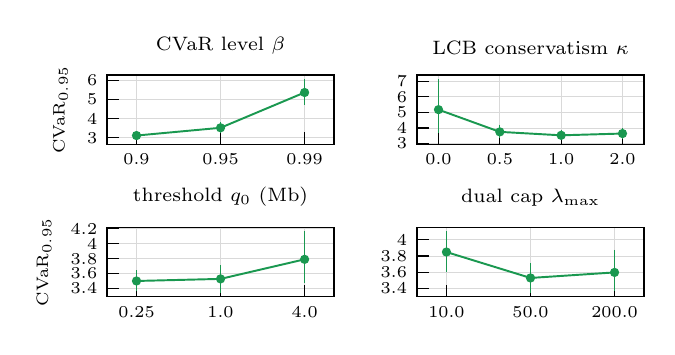
\begin{tikzpicture}
\begin{groupplot}[
  group style={group size=2 by 2, horizontal sep=30pt, vertical sep=30pt},
  width=82pt, height=25pt,
]
\nextgroupplot[title={CVaR level $\beta$},
  ylabel={$\mathrm{CVaR}_{0.95}$},
  xmin=-0.35, xmax=2.35,
  ymin=2.66677, ymax=6.27884,
  xtick={0,1,2}, xticklabels={0.9,0.95,0.99},
  xticklabel style={font=\fignote}, yticklabel style={font=\fignote},
  ylabel style={font=\fignote}]
\addplot[cproposed, mark=*, error bars/.cd, y dir=both, y explicit,
  error bar style={line width=0.4pt}, error mark options={line width=0.4pt, mark size=1pt}]
  table[x=x, y=y, y error plus=ep, y error minus=em] {
x y ep em
0 3.12315 0.100325 0.10683
1 3.52805 0.147835 0.146337
2 5.37017 0.559114 0.490408
};

\nextgroupplot[title={LCB conservatism $\kappa$},
  xmin=-0.35, xmax=3.35,
  ymin=2.95137, ymax=7.39823,
  xtick={0,1,2,3}, xticklabels={0.0,0.5,1.0,2.0},
  xticklabel style={font=\fignote}, yticklabel style={font=\fignote},
  ylabel style={font=\fignote}]
\addplot[cproposed, mark=*, error bars/.cd, y dir=both, y explicit,
  error bar style={line width=0.4pt}, error mark options={line width=0.4pt, mark size=1pt}]
  table[x=x, y=y, y error plus=ep, y error minus=em] {
x y ep em
0 5.17714 1.79076 1.3032
1 3.74923 0.283748 0.212734
2 3.52805 0.147835 0.146337
3 3.64203 0.189707 0.168778
};

\nextgroupplot[title={threshold $q_0$ (Mb)},
  ylabel={$\mathrm{CVaR}_{0.95}$},
  xmin=-0.35, xmax=2.35,
  ymin=3.29178, ymax=4.22107,
  xtick={0,1,2}, xticklabels={0.25,1.0,4.0},
  xticklabel style={font=\fignote}, yticklabel style={font=\fignote},
  ylabel style={font=\fignote}]
\addplot[cproposed, mark=*, error bars/.cd, y dir=both, y explicit,
  error bar style={line width=0.4pt}, error mark options={line width=0.4pt, mark size=1pt}]
  table[x=x, y=y, y error plus=ep, y error minus=em] {
x y ep em
0 3.50015 0.105569 0.100091
1 3.52805 0.147835 0.146337
2 3.79088 0.340262 0.281887
};

\nextgroupplot[title={dual cap $\lambda_{\max}$},
  xmin=-0.35, xmax=2.35,
  ymin=3.29889, ymax=4.1547,
  xtick={0,1,2}, xticklabels={10.0,50.0,200.0},
  xticklabel style={font=\fignote}, yticklabel style={font=\fignote},
  ylabel style={font=\fignote}]
\addplot[cproposed, mark=*, error bars/.cd, y dir=both, y explicit,
  error bar style={line width=0.4pt}, error mark options={line width=0.4pt, mark size=1pt}]
  table[x=x, y=y, y error plus=ep, y error minus=em] {
x y ep em
0 3.84876 0.223112 0.207935
1 3.52805 0.147835 0.146337
2 3.59648 0.244998 0.192829
};

\end{groupplot}
\end{tikzpicture}
\end{document}
